\documentclass[12pt]{article}
\usepackage{graphicx}

\linespread{1.5}
\addtolength{\oddsidemargin}{-2.5cm}
%\addtolength{\evensidemargin}{-3cm}
\addtolength{\textwidth}{2.5cm}
\begin{document}

\title{Making multiple-locus association mapping on a genome-wide scale routine}
\author{Andrew W. George and Joshua Bowden}

\maketitle


\abstract{Since the earliest of genome-wide association studies, a key shortcoming in how their data have been analysed has persisted. The strength of association between a marker locus and trait is measured for each locus separately, on a locus-by-locus basis. Multiple-locus methods that map multiple locus-trait associations simultaneously have been available for some time. However, they have attracted little attention. They can be demanding, computationally, and their results are not always easy to interpret. Yet, it is widely accepted that multiple-locus methods are superior, statistically, to locus-by-locus methods. Here, we present our method that makes the multiple-locus analysis of data from genome wide association studies routine. It is formulated within a linear mixed model framework. 
We call our method AMplus.  AMplus produces results faster than competing multiple-locus methods and often with greater statistical power. Also, it is just a little slower than the fastest single-locus linear mixed model implementations. 
AMplus is freely available as a fully documented R package. 
}



\section{Introduction}


Over the past decade,  Genome wide association studies have changed considerably in both their analysis and design. Early gwas followed a case-control design. Association mapping methods were no more complicated than contingency table tests or regression. These designs though had a tendency to yield spurious findings if there was unrecognised population stratification. This prompted a shift towards family-based designs and score tests, such as the tdt test and its variants (refs). Today, instead of by design, it is through statistical modelling that we account for the effects of population stratification. This has meant that data can be collected from general populations, even if these populations are highly structured. Analysis via sophisticated association mapping methods, such as linear mixed model based approaches,  is now almost routine.

What has not changed over the past decade is that it remains common practice to analyse gwas data on a locus by locus basis. This is despite there being several significant problems with analysing data in this way. First, the aim of association mapping is to identify regions of the genome that house genes that are influencing a trait. The identification of these regions from these analyses is not always straightforward. Gwas results are reported, typically, via Manhattan plots that plot the -log10 of the p value for each locus against the map position of the locus. The location of peaks in this plot signify regions of interest. Inferring the exact number of regions of interest can be difficult If the peaks are not well separated. Second, when multiple statistical tests are performed, the probability of wrongly accepting a significant result (type 1 error) is inflated. This is known as the multiple testing problem (refs). Many different solutions have been offered (refs). Yet, there is still no well accepted way of correcting for multiple testing in the context of genome- wide association mapping. Third, many of the traits whose genetic secretes we are trying to discover are complex. There will be multiple loci in linkage equilibrium with genes that influence the trait. Yet, A locus by locus mapping approach only assesses the evidence for association between a single marker locus and trait.

It is somewhat surprising then that multiple locus association mapping methods haven't attracted more attention. Methods based on 
regularisation techniques, such as ridge regression and lasso, measure all locus-trait associations simultaneously. 
Here, multiple testing is not an issue. These techniques though are computationally demanding. Also, their results can be difficult to interpret. The strength of association is not measured by a p-value but by the size of the regression coefficient for a locus in the model. More recently, associations have started to be mapped with random forests (refs). Similar to regularisation techniques though, it is not clear how to infer genomic regions of interest from their findings (refs). An multiple locus method that does show promise is the multi-locus linear mixed model method (ref). The best multiple locus model is built with simple variable selection. Results are immediately interpretable but here, computation can be a challenge for large data.

In this paper, we present our new multiple locus method for genome wide association mapping, which we are calling Eagle. Eagle combines the strength of regularisation techniques (being able to fit all locus-trait associations jointly), with simple variable selection (having easy to interpret results). Our method does not require a significance threshold to be set nor regularisation parameters to be fine tuned. Through a clever dimension reduction step, we are able to achieve a computational performance similar to the fastest single locus linear mixed model implementations. Eagle is statistically more powerful than single locus association mapping and is as and often more powerful than 
most multiple locus methods. Our aim is to make multiple locus association mapping on a genome wide scale routine. To this end, we have created a fully documented R package, that is easy to use, even for non R users.  Our package accepts marker data of different 
formats and can handle data larger than a computer's  memory capacity. It includes detailed error checking and makes heavy use of 
distributed computing for computation when available.  The purpose of this work was to make multiple-locus association mapping on 
a genome-wide scale, for large data sets,  practical and we have built AMplus accordingly. 


\section{Results}

\subsection{Association Mapping Methods}

We compared AMplus, in terms of computational and statistical performance, against seven other association mapping methods. 
We chose methods that had been purpose built for genome-wide analysis, that could handle data from quantitative traits, and where the methods had been implemented in freely available computer software. Two of the methods are based on single locus (or locus-by-locus) models and five are based on multiple locus models. Of the many ways of performing single locus association mapping, we chose GEMMA and FaST-LMM because of their popularity and computational speed. For multiple locus association mapping, we chose bigRR, glmnet, LMM-Lasso, MLMM, and r2VIM.  Each takes a different approach to mapping multiple locus-trait associations jointly.


From a practical perspective, how the methods were implemented, in terms of usability, varied greatly. In Table 1, we list seven important features for ensuring the usability of computer software for association mapping. We also identify which software has what features. 
In forming this list of features, we assumed that the primary purpose of a genome-wide association study is 
to identify the set of marker loci in true and strongest association with a trait.  The level of documentation varied across the implementations but only 
a few came with user manuals detailing the format of the input data and how to perform analyses. 
Most implementations could handle additional fixed effects which is important when accounting for hidden population structure. 
Few though could cope with marker data larger than the memory capacity of the computer. Similarly, few returned the best set of marker loci in strongest association with a trait as their result. Almost all the software returned results that required further processing, either 
by identifying the best set of marker loci via the setting of significance thresholds or having to do further analysis to calculate the significance of the results. Almost none of the association mapping software checked for errors in the input data.  Only AMplus has all seven features. 


\subsection{Computational Performance: run times and memory usage}


To asses the computational performance of AMplus, we conducted a large simulation study. 
We were interested in  the impact of study size on  performance so we generated data under five different scenarios. 
These are a GWAS of size 150 individuals and 5000 snp (150 X 5K), 350 individuals and 400000 snp (350 X 400K),  1500 individuals and 
50000 snp (1500 x 50K), 2000 individuals and 500000 snp (2000 x 500K), 4000 individuals and 
1500000 snp (4000 x 1.5M), and 10000 individuals and 1500000 snp (10000 x 1.5M).  
We chose these scenarios to reflect some of the different sized GWAS being performed in animals, plants, and humans. 
For each scenario, we generated 100 replicates of data. A single replicate consists of snp genotype data and quantitative trait data. 
We obtained the snp data from the publicly available 1000 genome project (phase 3). The quantitative trait data we generated from the 
snp data by selecting a set of snp loci, assigning allelic effects to these snp, and aggregating these effects for each individual along with 
random error. The number of snp selected per replicate follows a Poisson distribution with mean 30.
 The quantitative trait was generated to have a heritability of 50\%.
Analyses were performed on a high end desktop computer. It had dual 8-core Xeon processors, three Kepler Tesla GPUs, and 128 Giggabytes of RAM. All implementations except, GEMMA, made use of distributed computing, either explicitly or implicitly through multi-threaded BLAS/LAPACK libraries. 

\begin{figure}
\label{fig_runtimes}
\caption{Run times}
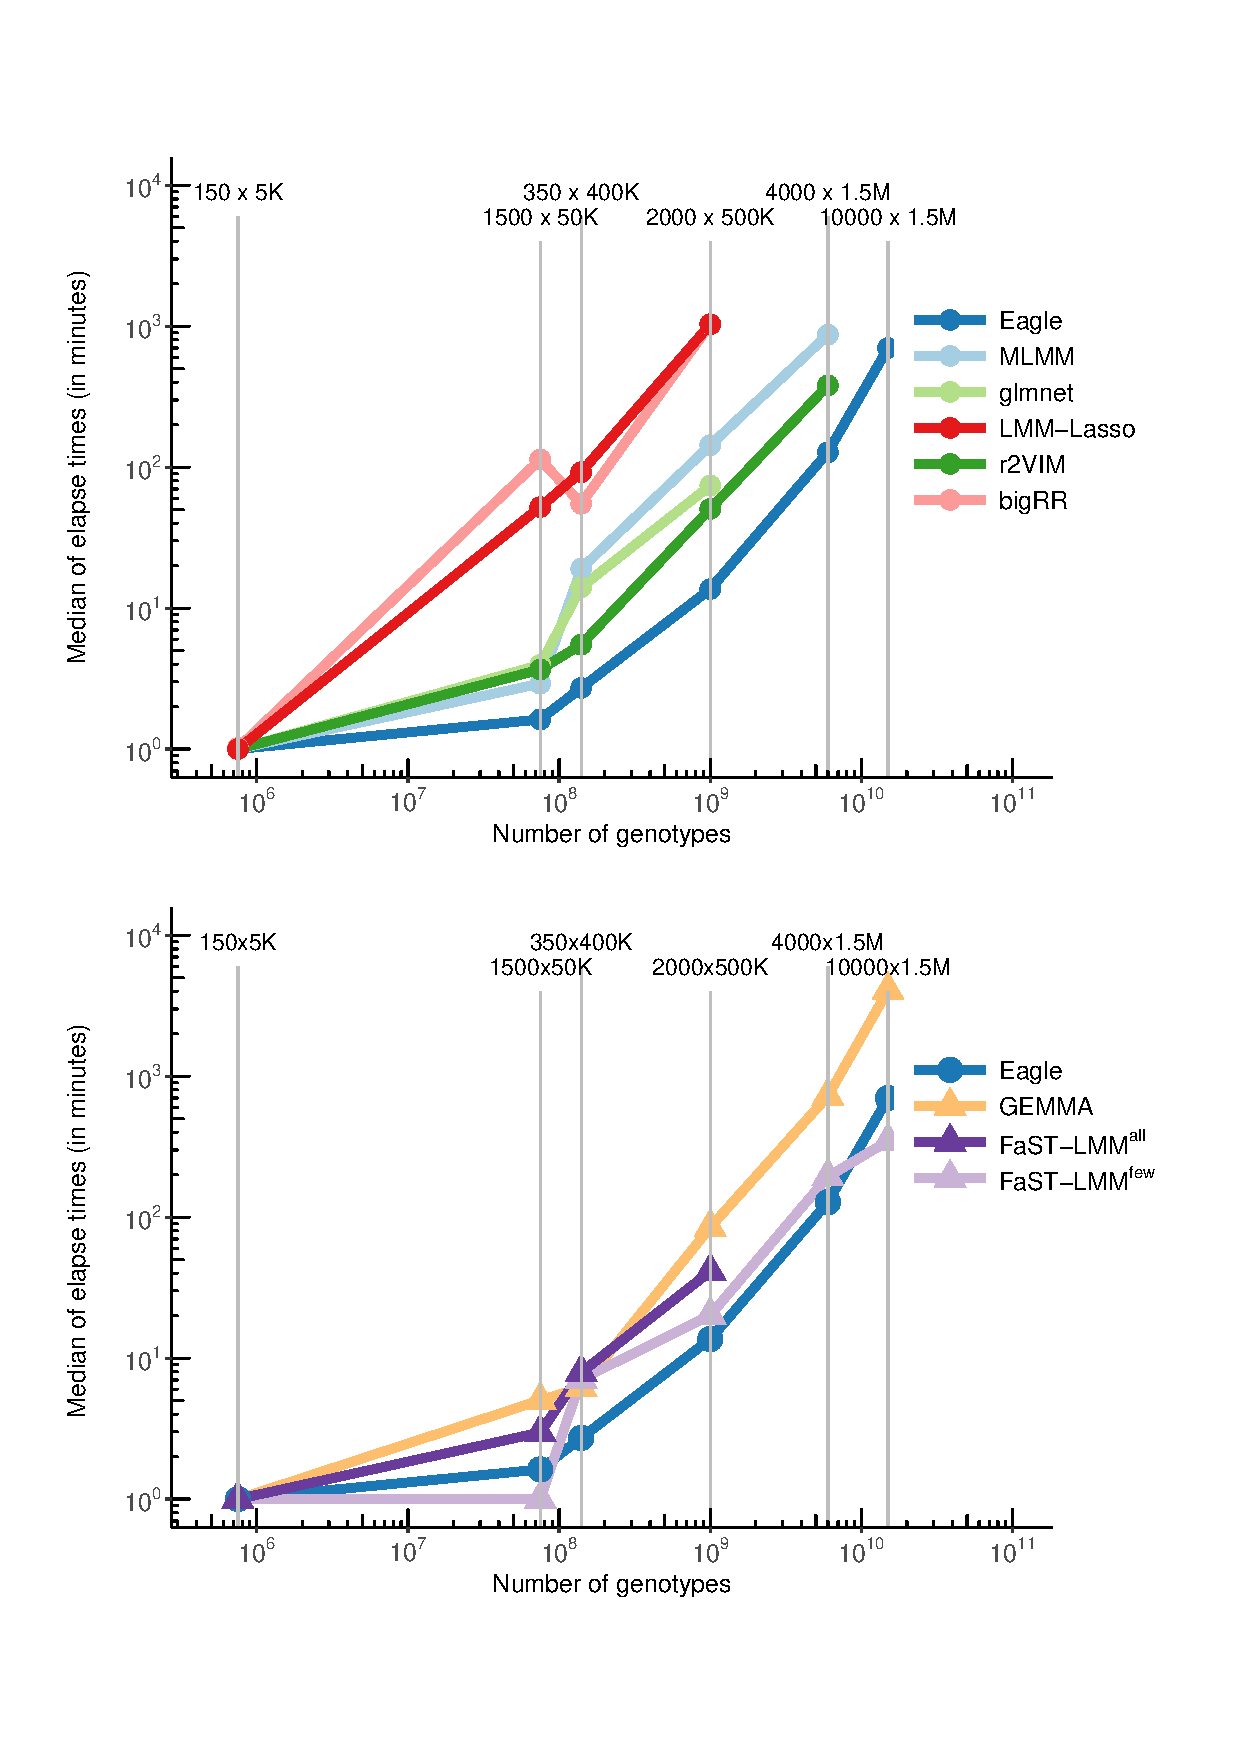
\includegraphics[width=10cm]{time}
\end{figure}


The run times for AMplus against the other software programs, across the five scenarios, is shown in figure \ref{fig_runtimes} To help with interpretibility of the results, in both plots, we have taken the x and y axes to be on a log scale. This means a unit change on the x or y axes is equivalent to a change in the order of magnitude. 
In the top plot, a point is the median of the ratios of elapse times of the multiple locus method to AMplus for a given scenario. The median is over the 100 replicates. Here, since the median of the ratios are all positive on the log scale, it means that AMplus had a shorter run time than than all the other multiple locus methods. In fact, in some cases, AMplus was over a hundred times, or over two orders of magnitude, faster. Unlike AMplus, the size of data under scenario 10000 X 1.5M was beyond the memory constraints of the other multiple locus implementations. This was also the case for LMM-Lasso, bigRR, and glmnet, for scenario 4000 x 1.5M.

In the bottom plot of figure \ref{fig_runtimes}, we compare the median run time of AMplus against the median run times of the single locus methods, FaST-LMM and GEMMA. 
FaST-LMM was run in two ways. It was run where the genetic similarity matrix was built with all the marker data (FaST-LMM$^all$) or with data on every 500th snp (FaST-LMM$^few$). 
AMplus was also run in two ways.  The default behavior for AMplus is to make use of CPUs for computing. However, AMplus also has the capacity to harness multiple GPUs (AMplus$^GPU$). 
From the bottom plot, all the implementations have short run times when analysing data from scenario 150x5K. However, for the other scenarios, AMplus and AMplus$GPU$ have 
significantly shorter run times than GEMMA and FaST-LMM$^all$. FaST-LMM$^few$ has a shorter run time than AMplus and AMplus$^GPU$ but only for scenarios 1500x50K and 
10000x1.5M.  Furthermore, for scenario 10000x1.5M, the median run time for GEMMA is 4071 minutes, for AMplus is 699 minutes, for AMplus$^GPU$ is 447 minutes, and for 
FaST-LMM$^few$ is 346 minutes. The very fast single-locus method FaST-LMM$^few$ is only 29\% faster than our multiple-locus method AMplus$^GPU$. It is worth noting though that 
there is a setup cost to accessing GPU computing, making AMplus$^GPU$ most efficient on the larger data. 


We also examined the memory usage of the different software programs (figure \ref{fig_memory} supplementary materials). 
AMplus is comparable to the most efficient single locus implementation, FaST-LMM$^few$. 
AMplus is also the only multiple locus program able to analyse data under scenarios ..... and ..... . 
AMplus can process data larger than the memory capacity of the computer.

\begin{figure}
\label{fig_memory}
\caption{Memory usage}
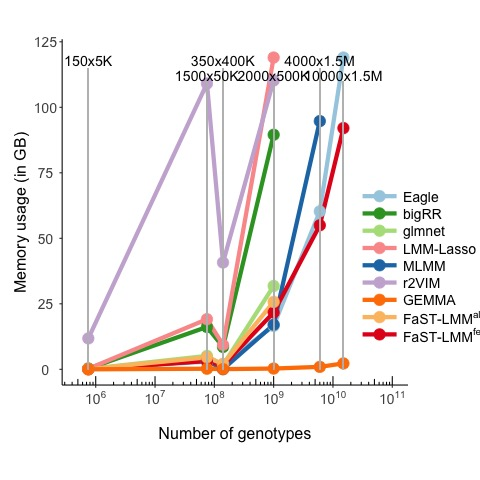
\includegraphics[width=10cm]{mem}
\end{figure}




\subsection{Statistical Performance: power, FDR, and significance thresholds}

As part of assessing the performance of AMplus against the other association mapping methods, 
we calculated their statistical power and false discovery rates. 
We want a method to have high statistical power (probability of finding a true positive finding) but 
low false discovery rate (proportion of findings that are false positives). 
All the methods, besides AMplus and MLMM, required a threshold to be set in order to identify significant findings. 
A conservative threshold guards against false discoveries but reduces power. 
A anti-conservative threshold increases power at the cost of also increasing the false discovery rate. Only AMplus and mlmm avoid thresholds by treating association mapping as a model selection problem where the best model is found by minimising the model selection statistic, extBIC.

Figures \ref{fig_power_multiple}  and \ref{fig_power_single} show the relationship, calculated empirically, between the power and fdr for each method. The multiple-locus (Figure \ref{fig_power_multiple})   and the single-locus (Figure \ref{fig_power_single})  methods are plotted separately for clarity. 
AMplus features in both plots for comparison. By varying the significance thresholds for the different methods, we were able to calculate the change in power and fdr. Since AMplus and MLMM do not rely on thresholds, their power and fdr appear as single points in the plots. In practice, the true power and fdr is unknown. However, because we generated data where we knew which loci were acting as quantitative trait loci, we were able to calculate the true power and fdr for the methods.

From figures \ref{fig_power_multiple}  and \ref{fig_power_single}, the superior performance of AMplus is apparent. When the fdr is low, AMplus has the highest power with Mlmm also performing well. AMplus is noticeably more powerful than the single locus methods. 
It is possible to set a significance threshold for these other methods that results in higher power. 
However, this comes at the cost of an intolerably high fdr.

For the methods evaluated here that require a significance threshold, figure  \ref{fig_threshold}  shows how 
threshold size impacts fdr. Each plot corresponds to the results from a different method. 
A curve within a plot is formed from analysing data with the method and using different threshold values to identify locus-trait associations. 
The true fdr is then calculated from these findings.
We can see from figure \ref{fig_threshold}  that the threshold impacts the fdr differently across methods. The relationship between threshold value and fdr even differs when data are analysed with the same method but for different scenarios. This demonstrates one of the challenges in using association mapping methods that are reliant upon thresholds. With AMplus, we do not have this challenge. For completeness, for the small sampled size scenarios ... And ....., the fdr for AMplus was 0.07 and 0.09, respectively. With the larger study sizes of ..., ..., and ...., the fdr drops to ..., .., and ..... respectively.


\begin{figure}
\label{fig_power_multiple}
\caption{Power curves for  multiple locus methods}
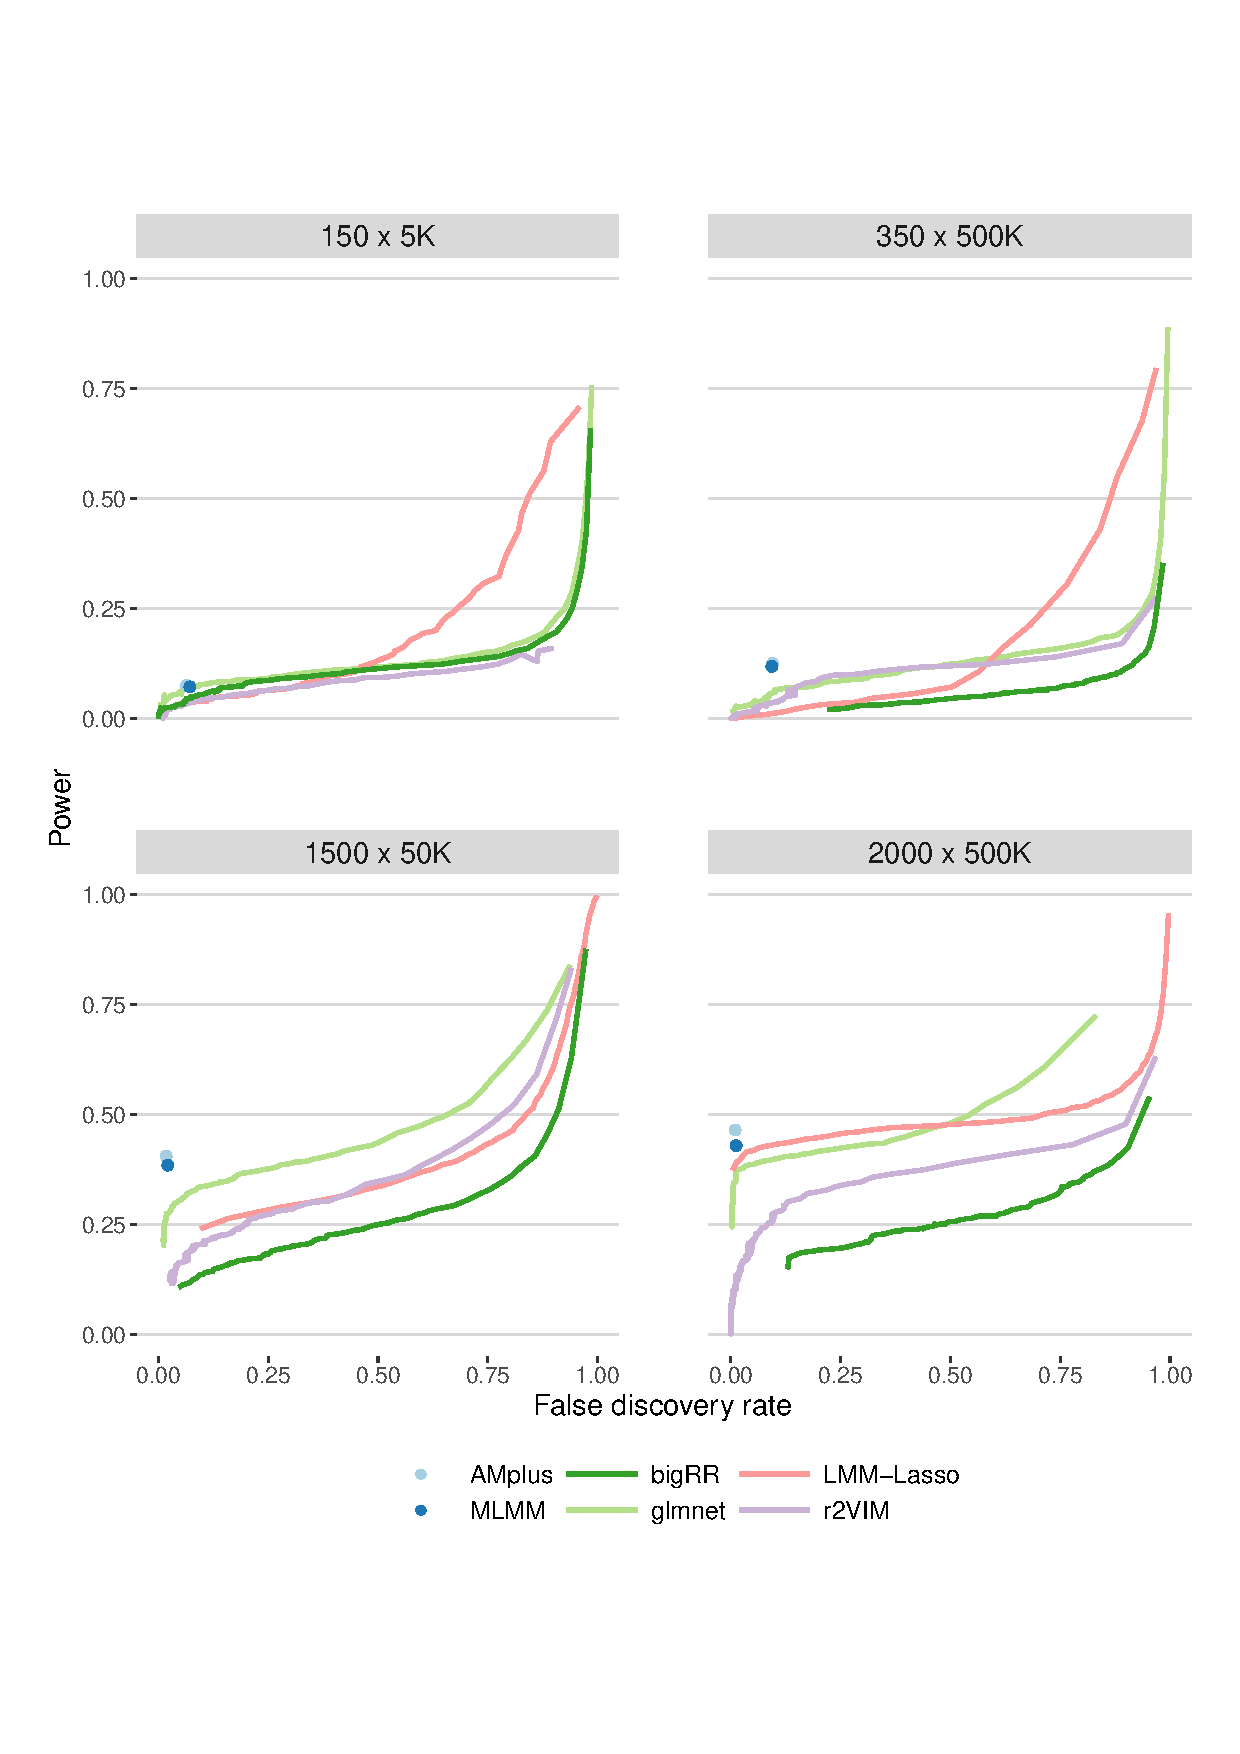
\includegraphics[width=10cm]{powerMultiple}
\end{figure}

\begin{figure}
\label{fig_power_single}
\caption{Power curves for single-locus methods -- Put into sup methods}
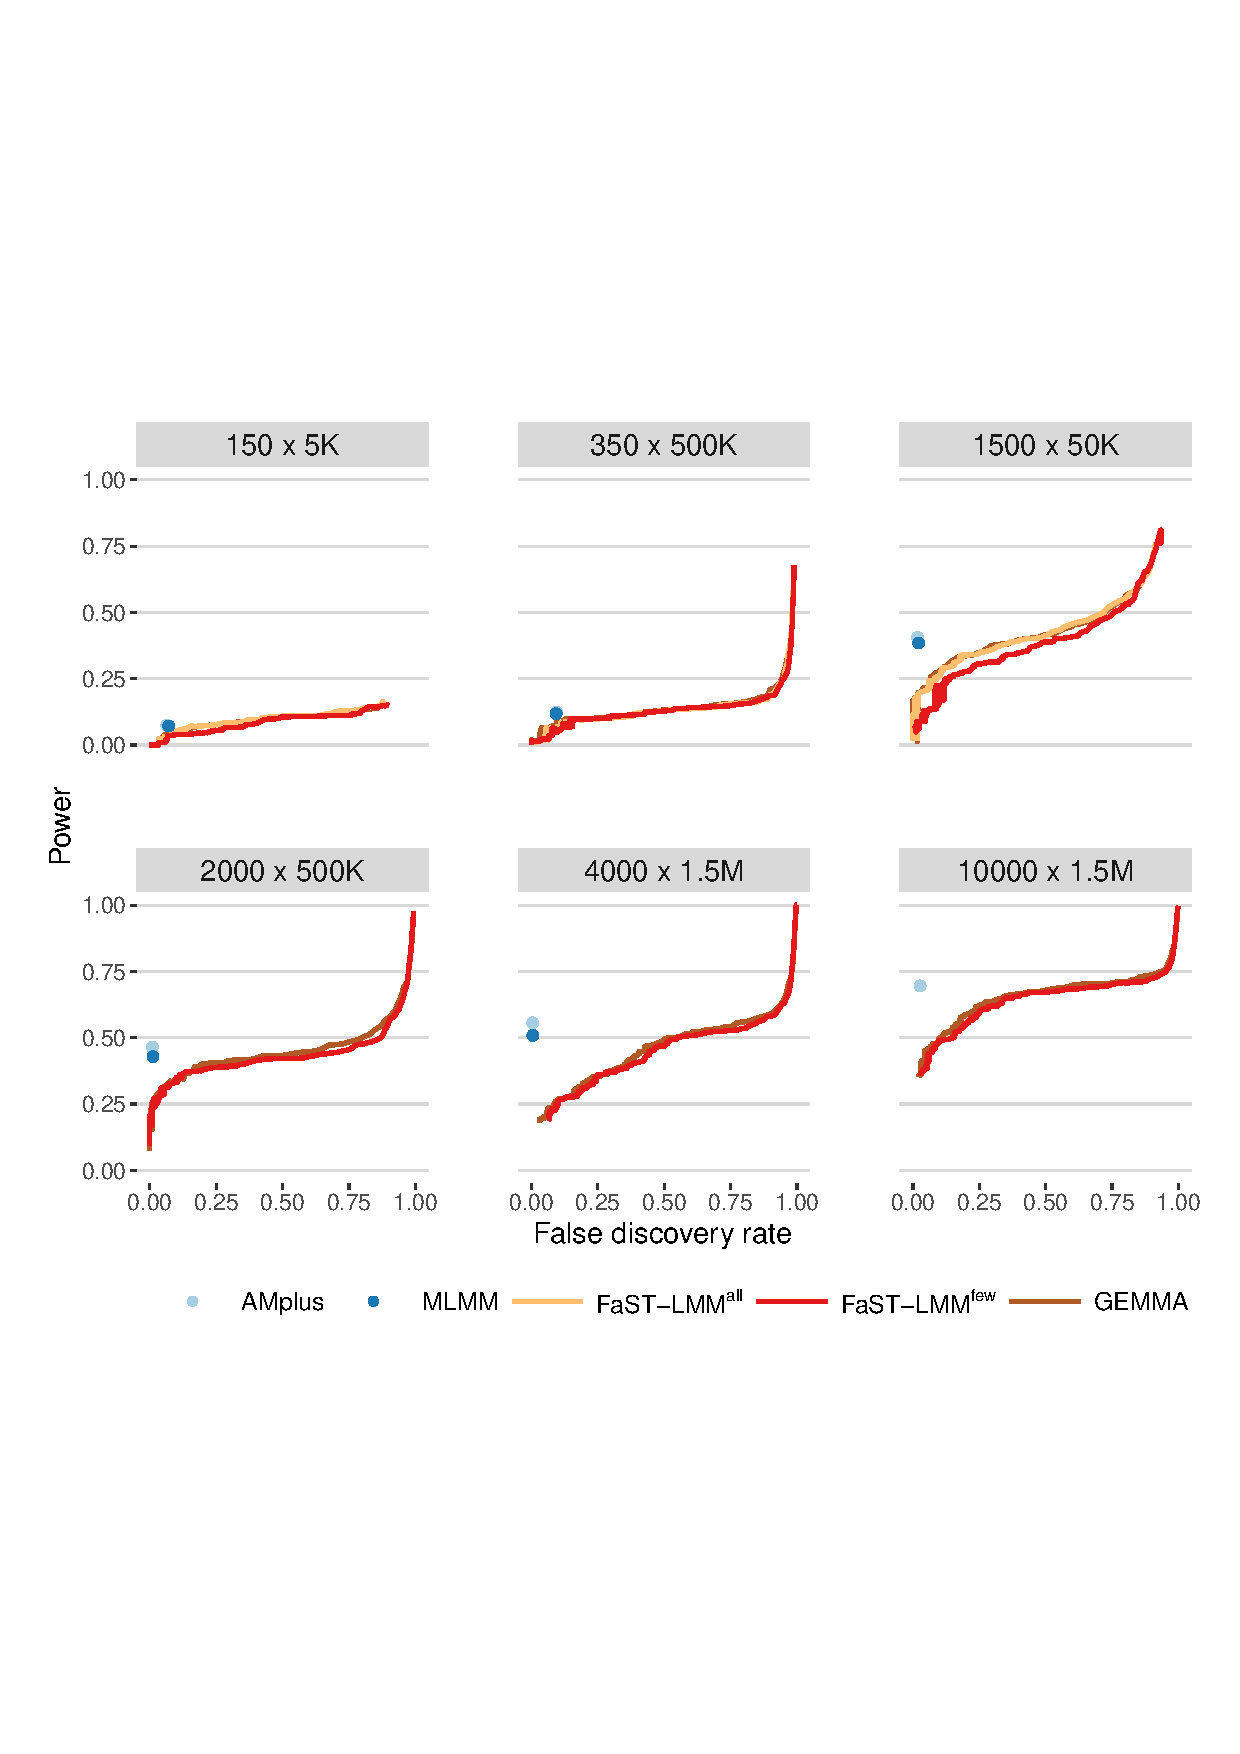
\includegraphics[width=10cm]{powerSingle}
\end{figure}


\begin{figure}
\label{fig_threshold}
\caption{The impact of threshold on FDR }
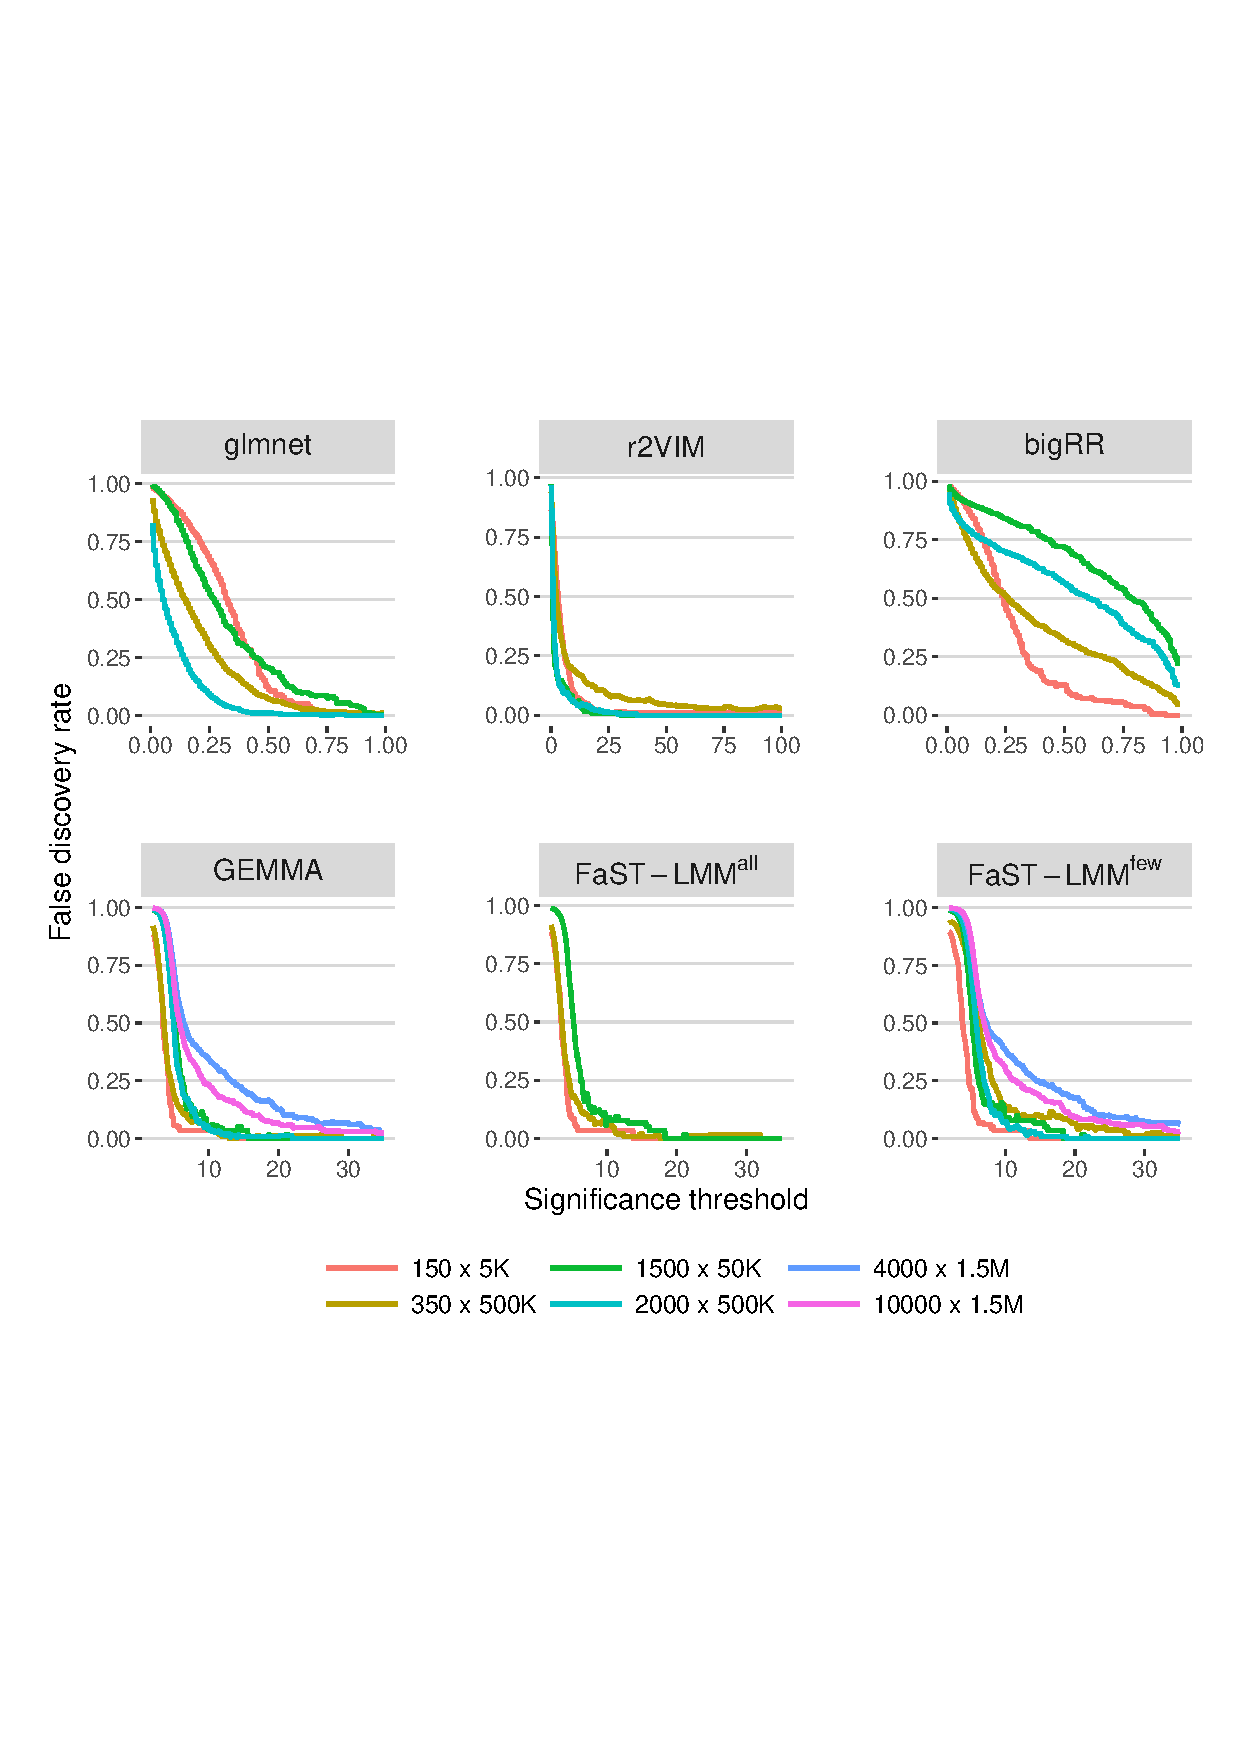
\includegraphics[width=10cm]{threshold}
\end{figure}




\subsection{Mouse Study}

\section{Methods}

\subsection{Outbred Mice Study}

Phenotypic and genotypic data were collected on a large study population of commercially 
available outbred mice. The aim of the study was to map, through association, the genetic basis
of complex traits in mice. The construction of the population and collection of data are described in detail in 
\cite{Nicod:2016aa}.  Briefly, the population consists of 2073 adult outbred mice from Charles River Laboratories. Phenotypic data
were obtained from 200 traits. These traits fell into the categories of behaviour, tissue, and physiology. Genotype 
data were collected from 7, 073, 398 SNPs.  A reduced set of 359, 559 SNP across the 19 
autosomes and sex chromosome was then identified, upon which all genome-wide analyses were based.  These SNP tagged all other SNP with MAF $> 0.1\%$
and LD $r^2 > 0.98$.  Missing data?

\subsection{Eagle Approach for Multiple-locus Association Mapping}
\subsubsection{Overview}


Eagle is an approach that identifies genomic regions of interest for a trait via the building of a (linear mixed) model. The model is built iteratively, without need of significance levels or thresholds. The model has two parts, a fixed effects part and a random effects part. The random effects part contains the error and an effect for the snp-trait association across the entire genome. It is from this effect 
 that we are able to identify which snp is in strongest association with the trait.  
 Our model building process is as follows. First we fit the current model to the data. Second, from the random effect for association, we identify which snp is in strongest association  with the trait.  Third, we move this snp from the random effects to the fixed effects.
We do this to stop the neighbours of the chosen snp from being selected in subsequent iterations and 
to give opportunity to snp in linkage disequilibrium with genes having lesser impact on the trait to be discovered. 
 Fourth, we calculate if the new model is "better" than the current model. 
If so,  the new model becomes the current model and we repeat the process.   Once the model building process is complete, the findings from Eagle are the set of snp that have been moved into the fixed effects part of the model.  These snp map the seperate regions of the genome that house genes that are influencing the trait.  
 
 
 
 

\subsubsection{The specifics}
The Eagle approach for multiple-locus association mapping is based on building a linear mixed model, iteratively, via forward 
selection.  Suppose $s$ iterations of our model building process have already been performed. 
The next iteration is performed as follows. First, we fit the current model to the data. The model is of the form 
\begin{equation}
y = X \tau + u_g + e
\end{equation}
where $y^{(n \times 1)}$ is a vector containing the quantitative trait values observed from $n$ individuals, 
$X^{(n \times p)}$ is a known design matrix of full rank, 
$\tau^{(p \times 1)}$ is a vector of $p$ fixed effects parameters, 
$u_g^{(n \times 1)}$ is a vector 
of genetic effects, and 
$e^{(n \times 1)}$ is a vector of residuals whose distribution is assumed to follow $N(0, \sigma^2_e I^{(n \times n)})$. 




Suppose phenotypic and genotypic data are collected from a genome-wide association study involving $n$ individuals. 
Let $Y^{(n \times 1)}$ be a vector containing the quantitative trait data. Also, let $M^{(n \times L)}$ be a matrix of snp genotypes which have been collected from the $n$ individuals across $L$ snp loci. $M$ contains values -1, 0, and 1 corresponding to snp genotypes AA, AB, and BB, respectively. 

To identify genomic regions which contain genes that influence the trait 

We map genomic regions containing genes that influence the trait 




Suppose $s$ iterations have been performed of our multiple locus association mapping algorithm. This means $s$ snp-trait 
associations of significance have been identified. It also means $s$ separate regions containing putative genes 
that influence the trait have been mapped.  To find perform iteration $s+1$ and the next snp, we perform the following steps.  First, 



Let $M^{(n \times L} $be a matrix of snp genotypes which have been collected from the n individuals across L snp loci. These L loci are assumed to span the entire genome. M contains values -1, 0, and 1 corresponding to snp genotypes aa, ab, and bb, respectively. 

S={S1,...Ss} be 








Our model building process is as follows.  Suppose $s$ SNP have already been found. First we fit the current model to the data.




Suppose our iterative model building procedure has already found $s$ snp. Then

Our linear mixed model for multiple-locus association mapping, given trait data $y^{(n \times 1)}$ which are collected on $n$ individuals, 
is of the form 
\begin{equation}
y = X \tau + u_g + e
\end{equation}
where $X^{(n \times p)}$ is a known design matrix of full rank, $\tau^{(p \times 1)}$ is a vector of fixed effects parameters, $u_g^{(n \times 1)}$ is a vector 
of genetic effects, and $e^{(n \times 1)}$ is a vector of residuals whose distribution is assumed to follow $N(0, \sigma^2_e I^{(n \times n)})$. 

Now, let $M^{(n \times L)}$ be a matrix of genotypes collected from $L$ snp.  The 
matrix contains the values -1, 0, and 1, corresponding to the snp genotypes AA, AB, and BB, respectively.  It is assumed that 
missing genotypes have been imputed. 

Suppose $s$ SNP have already been found. 


$S={ S_1, S_2, \ldots, S_s}$ be the set of column indexes 




\bibliographystyle{nature}
\bibliography{bibcitelibrary}

\end{document}
